% headsectionstart
% update mixedReport hedsection if any changes done in this headsection
\documentclass{article}
\usepackage[a4paper, margin={40pt, 40pt}]{geometry}
\usepackage{tikz}
\usepackage{pgfplots}
\usepackage{pgf-pie}
\usepackage{adjustbox}
\usepackage[T1]{fontenc}
\usepackage{minted}
\usepackage[colorlinks = true,
linkcolor = blue,
urlcolor  = blue,
citecolor = blue,
anchorcolor = blue]{hyperref}
\usepackage[outline]{contour}
\contourlength{1pt}

\usetikzlibrary{fit,backgrounds,positioning,decorations.markings,shapes,arrows,shadows}
\definecolor{primary}{RGB}{115,54,163}
\definecolor{theftBgColor1}{RGB}{235,215,249}
\definecolor{theftBgColor2}{RGB}{238,229,197}
\definecolor{theftValueType1Color}{RGB}{0,0,0}
\definecolor{theftValueType2Color}{RGB}{115,54,163}
\definecolor{theftValueType3Color}{RGB}{125,110,142}
\definecolor{yesVoteColor}{RGB}{115,54,163}
\definecolor{noVoteColor}{RGB}{61,38,80}
\definecolor{yesNoBarBgColor}{HTML}{EDEDED}
\definecolor{yesNoBarBorderColor}{HTML}{B2AEAE}
\definecolor{noProgressBgColor}{HTML}{E26C6C}

\tikzset{
	headerText/.style={text=white},
	fullWidth/.style={text width=480pt},
  yesNoBar/.style={minimum width=101pt, minimum height=30pt},
	yesNoBarBg/.style={yesNoBar, draw=yesNoBarBorderColor, fill=yesNoBarBgColor, rounded corners=3pt, line width=1pt, right},
	yesNoBarProgress/.style={yesNoBar, fill=primary, minimum height=29pt, rounded corners=2.5pt, right= -101.25pt, inner sep=0},
	yesNoBarText/.style={yesNoBar, right, white, right= -101.25pt},
	leftHeaderText/.style={headerText, align=left,text width=280pt},
	rightHeaderText/.style={headerText, align=right,text width=180pt},
	theftBlock/.style={rounded corners=5pt, inner sep=10pt},
	theftBlockContent/.style={text=black, text width=100pt},
	isTheftBlock/.style={align=left, text width=120pt}
}

\begin{document}
\sffamily
% headsectionend

\hypertarget{--pageID--}{}
% header
\trimbox{0 -15pt 0 0}{ 
  
\begin{tikzpicture}
      \node[leftHeaderText] (subtitle) {ZeroTheft Movement: --subtitle--};
      \node[leftHeaderText, below=of subtitle, below=5pt] (title) {\huge \textbf{--title--}};
      \node[leftHeaderText, below=of title, below=-5pt] (belowtitle) {voted theft Ethically, not legally};

      \node[rightHeaderText, right=10pt of subtitle] (year) {--year--};
      \node[rightHeaderText, below=of year, below=5pt] (country) {for --country--};
      \node[rightHeaderText, below=of country, below=5pt] (holon) {\href{--holonUrl--}{\color{white}--holonUrl--}};
    
      \begin{scope}[on background layer]
      \node[fill=primary, fit=(subtitle)(title)(belowtitle)(year)(country)(holon)] (header) {};
      \end{scope}
  \end{tikzpicture}
}

\trimbox{-120pt -15pt 0 0}{ 
  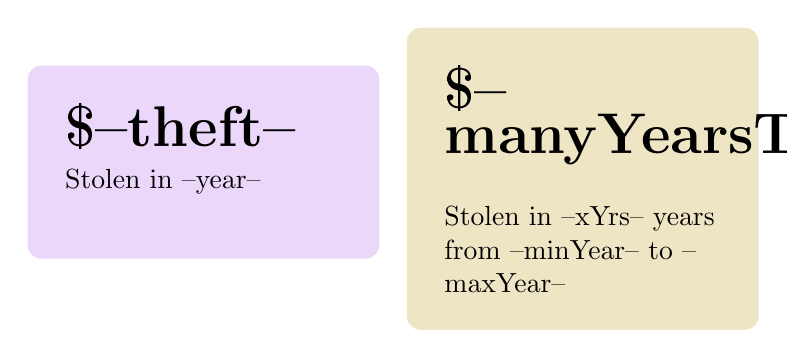
\begin{tikzpicture}
      \node[theftBlockContent] (amount1) {\huge \textbf{\$--theft--}};
      \node[theftBlockContent, below=0ptof amount1] (year1) {Stolen in --year--\newline};
      
      \begin{scope}[on background layer]
      \node[theftBlock, fill=theftBgColor1, fit=(amount1)(year1)] (block1) {};
      \end{scope}

      \node[theftBlockContent, right=30ptof amount1] (amount2) {\huge \textbf{\$--manyYearsTheft--}};
      \node[theftBlockContent, below=0ptof amount2] (year2) {Stolen in --xYrs-- years\\from --minYear-- to --maxYear--};
      
      \begin{scope}[on background layer]
      \node[theftBlock, fill=theftBgColor2, fit=(amount2)(year2)] (block2) {};
      \end{scope}
  \end{tikzpicture}
}

\trimbox{25pt -40pt 0 0}{
  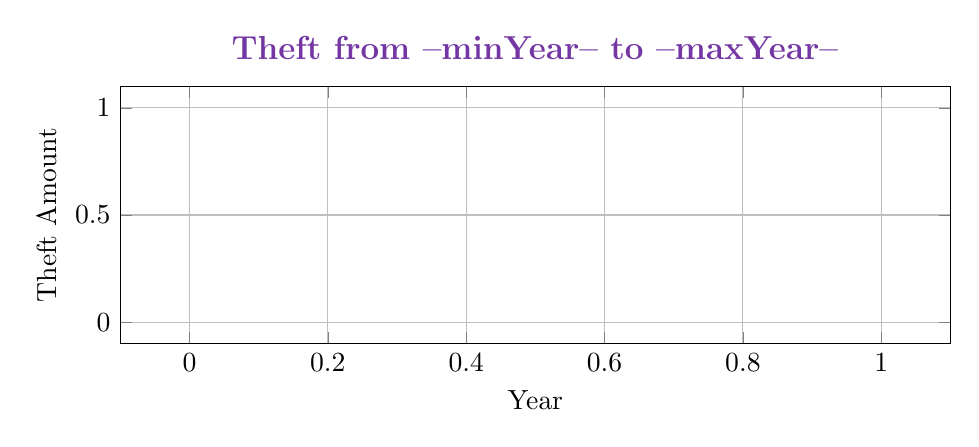
\begin{tikzpicture}
    \begin{axis}[
      title style={at={(0.5,1)},anchor=south,text=primary},
      title = \large \textbf{Theft from --minYear-- to --maxYear--},
      xlabel={Year},
      ylabel={Theft Amount},
      % xmin = 0, xmax = 10,
      % ymin = 0, ymax = 1,
      grid = both,
      % xtick distance = 1,
      x tick label style={/pgf/number format/.cd,%
        scaled y ticks = true,
        set thousands separator={},
        fixed},
      width = \textwidth,
      height = 0.4\textwidth,
      legend cell align = {left},
      % legend pos = north west,
      legend style={at={(0.5,-35pt)},anchor=north},
      scatter/classes={
      voting={theftValueType1Color, /tikz/mark size=3pt},%
      incompletevoting={theftValueType2Color, /tikz/mark size=3pt},%
      estimation={theftValueType3Color, /tikz/mark size=3pt}}
    ]
    
    \addplot[
      scatter,mark=*,primary,
      text=primary,
      scatter src=explicit symbolic,
      nodes near coords*=\scriptsize \textbf{\Theft},
      every node near coord/.append style={below right, rotate=90, shift={(0, 6pt)}},
      visualization depends on={value \thisrow{Theft} \as \Theft},
    ] 
    table [meta=DeterminedBy] {
      --theftValueChartData--
      % Year theft DeterminedBy Theft
      % 1    0.3  voting       0.25T   
      % 2    0.1  estimation       1.5    
      % 3    0.6  voting      0.70   
      % 4   0.4  incompletevoting      0.125  
      % 8   0.1  estimation       2      
    };
    
    \legend{
      % voting
      Voted Theft, 
      % incompletevoting
      Interim Theft (needs more vote),
      % estimation
      Estimated Theft
    }
    
    \end{axis}
  \end{tikzpicture}
}

\trimbox{0 -40pt 0 0}{
  \begin{tikzpicture}[scale=1.5, transform shape]
    \node[isTheftBlock, primary] (isTheft) {\Large \textbf{IS THIS THEFT?}};
    \node[below=5pt of isTheft, isTheftBlock] (noOfVoters) {\scriptsize Total No of Voters: --totalVotes--};
    \node[below=-4pt of noOfVoters, isTheftBlock] (votedYesNo) {\scriptsize Voted Yes: --yesVotes-- \quad Voted No: --noVotes--};

    \node[yesNoBarBg, yshift=-30pt, left=-105pt of votedYesNo] (yesBg) {};
    % \node[right=of yesBg, yesNoBarProgress, minimum width=75pt] (yesBar) {};
    \node[right=of yesBg, yesNoBarProgress, minimum width= --yesVotePercent--pt] (yesBar) {};
    \node[right=of yesBg, yesNoBarText] (yesPercent) {\contour{black}{\LARGE \textbf{Yes --yesVotePercent--\%}}};
 
    \begin{scope}[on background layer]
      \node[fit=(yesBg)(yesBar)(yesPercent), inner sep=0] (yesGraph) {};
    \end{scope}

    \node[yesNoBarBg, below= 10pt of yesBg] (noBg) {};
    % \node[right=of noBg, yesNoBarProgress, minimum width=0pt, noProgressBgColor] (noBar) {};
    \node[right=of noBg, yesNoBarProgress, minimum width= --noVotePercent--pt, noProgressBgColor] (noBar) {};
    \node[right=of noBg, yesNoBarText] (noPercent) {\contour{black}{\LARGE \textbf{No --noVotePercent--\%}}};
 
    \begin{scope}[on background layer]
      \node[fit=(noBg)(noBar)(noPercent), inner sep=0] (noGraph) {};
    \end{scope}
  \end{tikzpicture}
}
\trimbox{-10pt 20pt 0 0}{
  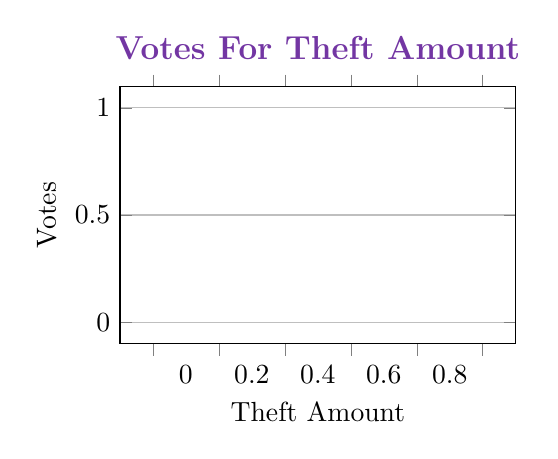
\begin{tikzpicture}
    \begin{axis}[
      ybar interval,
      title style={at={(0.5,1)},anchor=south,text=primary},
      title = \large \textbf{Votes For Theft Amount},
      xlabel={Theft Amount},
      ylabel={Votes},
      ymajorgrids = true,
      xmajorgrids = false,
      width = 0.545\textwidth,
      height = 0.4\textwidth,
      xtick = {}
    ]
      \addplot[draw=none,fill=primary] table
        {
          --votesForTheftAmountData--
          % Theft Votes
          % 1000    10
          % 1200    20
          % 1300    5
          % 1500   15
          % 2000   20
          % 2100   30
        };
    \end{axis}
    \end{tikzpicture}
}

\newpage 
\trimbox{0 -15pt 0 0}{ 
  
\begin{tikzpicture}
    \node[fullWidth, text=primary] (leadingProposal) {\huge \textbf{Leading Proposals}};
    \node[fullWidth, below =0ptof leadingProposal] (viewProposalTextLink) {\href{--holonUrl--/path/--pathSlug--/issue/--leafSlug--}{\color{blue}View Full Proposal Text}};
    \node[fullWidth, below =0ptof viewProposalTextLink] (leadingProposalTitle) {\large \textbf{Proposal ID --leadingProposalID-- by --leadingProposalAuthor-- on --leadingProposalDate--}};
  \end{tikzpicture}
}

\noindent
  \begin{minted}[%
    breaklines,
    mathescape,
    numbersep=5pt,
    numbersep=5pt,
    xleftmargin=0pt,
    xrightmargin=0pt,
    breaksymbolleft=,
    gobble=0,
    linenos
  ]{yaml}
--leadingProposalDetail--
  \end{minted}

  --viewMore--
\end{document}
